\documentclass{report}
\usepackage[a4paper, margin=0.5in]{geometry}
\usepackage{parskip}
\usepackage{graphicx}
\usepackage{caption}
\usepackage{amssymb}
\usepackage{amsmath}
\usepackage{algpseudocode}
\usepackage{algorithm}

\captionsetup[figure]{
  font = it,
  labelfont = bf
}

\begin{document}
\begin{minipage}[b]{0.48\textwidth}
  \section*{Algorithm testing}
  What has been described up to this point allows to create a parallel kmeans clustering which exploit the Hamerly's algorithm. In this section we present the result some tests that have been done using the Lloyd, Hamerly and parallelized Hamerly algorithm to compare the performances.

  \section*{General testing methodology}
  For every of the following tests has been used the same procedure.

  For each of the presented datasets, first a lloyd model is initiated and executed to set a reference time which is then used to measure the speedup of the hamerly algorithm with 1 to 10 threads. 
  
  The speedup is calculated as
  \begin{equation}
    speedup = 1 - \frac{hamerly\_time_T}{lloyd\_time}
  \end{equation}

  where $hamerly\_time_T$ is the time taken by the hamerly algorithm with T threads.

  For every model, a fixed number of iterations (100) has been used to stop the respective algorithm after the same number of updates.
  
  \section*{Randomly generated dataset }
  The first dataset is a randomly generated one which allows to easily study how the algorithm scales over N, K and D because it is simple to implement an algorithm which increments one of the three while keeping fixed the other 2.

  \subsubsection*{Points scaling}
  To scale over N, the testbench starts from a dataset with 3 centroids and a dimensionality of 2 while the number of points goes from 500 up to 50000. Figure \ref{fig:lh123_3Drnd} shows the testbench result.

  \begin{center} 
    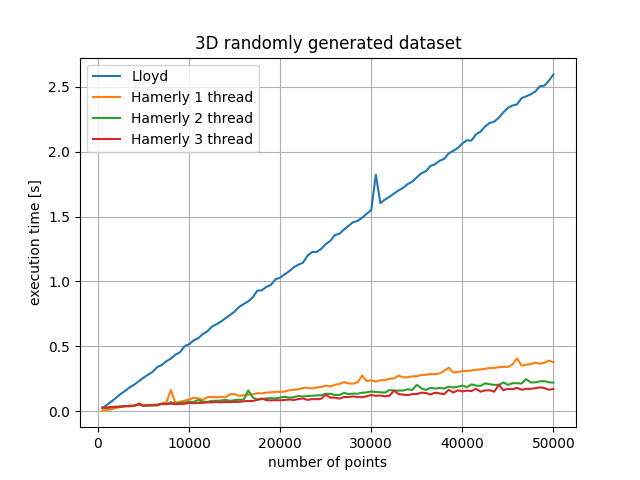
\includegraphics[width = 1\textwidth]{imgs/lh123_3Drnd.png}
    \captionof{figure}{result of the test on the 3D randomly generated dataset scaling over N}
    \label{fig:lh123_3Drnd}
  \end{center}

  The result, for each model, is a straight line which can also be proven mathematically because if the number of centroids and the dimensionality are constants (fixed numbers) then, from equation \ref{eq:hameq} and \ref{eq:lloydeq}, it is possible to factor N out which results in a straight line equation (y = mx).

\end{minipage}
\hspace{0.1in}
\begin{minipage}[b]{0.48\textwidth}


  \subsubsection*{Centroids scaling}
  The second testbench scales over K. Therefore, the testbench has a fixed number of points (3000) and dimension (3) while the centroids goes from 2 up to 100. Figure \ref{fig:lh123_3Drnd_cent} shows the result of the testbench.

  \begin{center} 
    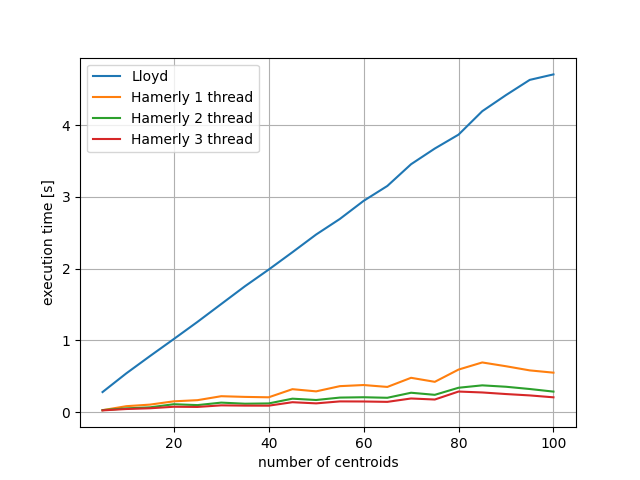
\includegraphics[width = 1\textwidth]{imgs/lh123_3Drnd_cent.png}
    \captionof{figure}{result of the test on the 3D randomly generated dataset scaling over K}
    \label{fig:lh123_3Drnd_cent}
  \end{center}

  Since K can be factored out from equations \ref{eq:hameq} and \ref{eq:lloydeq} when N and D are fixed, we see a straight line patter for each model.
  
  \subsubsection*{Dimension scaling}
  Lastly, to study how the algorithm scales over D, this dataset has a fixed number of points (3000), a fixed number of centroids (3) while the dimensionality of the data goes from 2 up to 100. Figure \ref{fig:lh123_3Drnd_dim} show the result of the testbench.

  \begin{center} 
    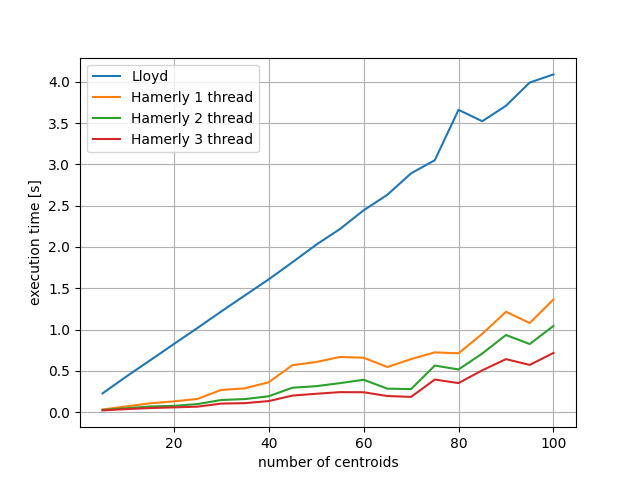
\includegraphics[width = 1\textwidth]{imgs/lh123_3Drnd_dim.png}
    \captionof{figure}{result of the test on the randomly generated dataset scaling over D}
    \label{fig:lh123_3Drnd_dim}
  \end{center}

  \subsubsection*{Speedup}
  To summarize the results, Figure \ref{fig:speedup} shows the speedup line for each of the previous graphs. In the latter it can be seen that the line corresponding to the D scaling has the lowest overall speedup but it is also the one where increasing the number of threads produces the most speedup, in other words, in this case, it is the one where using more threads is most effective.
  

\end{minipage}

\newpage

\begin{minipage}[b]{0.48\textwidth}

  \begin{center} 
    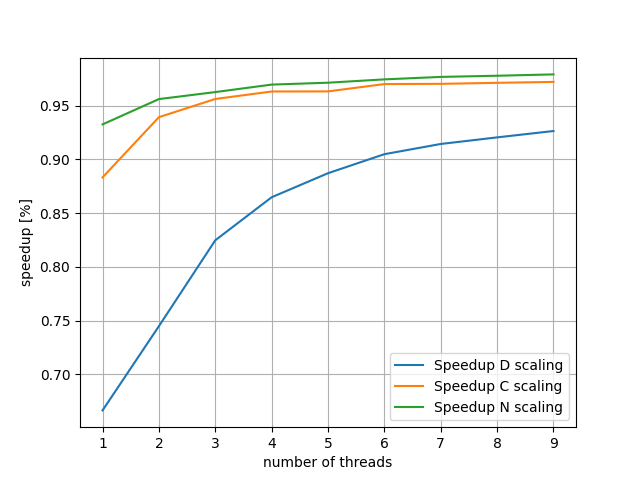
\includegraphics[width = 0.9\textwidth]{imgs/rndspeedup.png}
    \captionof{figure}{overall speedup on the random dataset}
    \label{fig:speedup}
  \end{center}

  \section*{Wine quality dataset}
  To test the algorithm with a more realisitc dataset, we downloaded\footnote{https://www.kaggle.com/datasets/yasserh/wine-quality-dataset} a dataset which contains features about different wines which can be used to group them in classes representing their quality between 0 and 10.

  The number of points in the dataset is 1143, with a dimensionality of 11. The centroids are 10 and were generated by randomly select them between the whole dataset.\\

  This dataset has been tested by scaling the points N starting from 9 up to 1143. Figure \ref{fig:lh123_wine} shows the result of the execution.

  \begin{center} 
    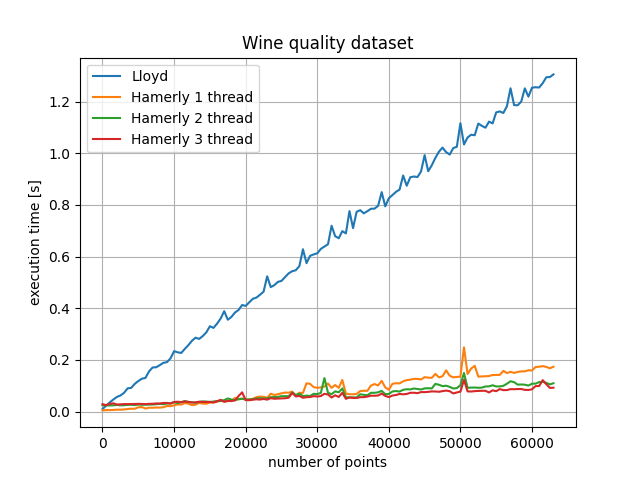
\includegraphics[width = 0.8\textwidth]{imgs/lh123_wine.png}
    \captionof{figure}{result of the test on wine dataset}
    \label{fig:lh123_wine}
  \end{center}

  \subsubsection*{Speedup}
  Figure \ref{fig:lh123_wine_speedup} shows the speedup of the algorithm when scaling both for N and D.
  \begin{center} 
    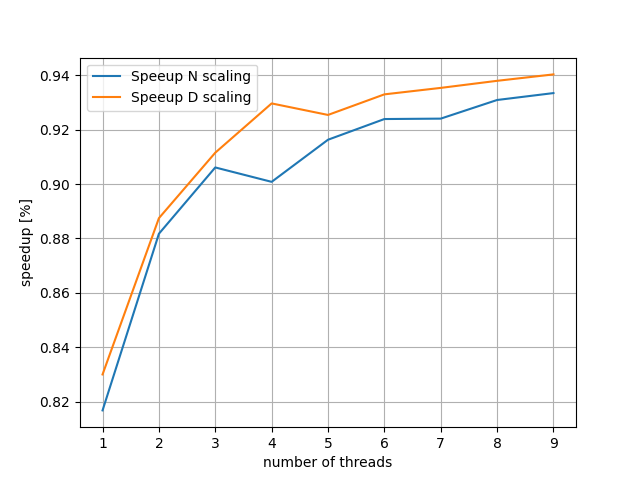
\includegraphics[width = 0.8\textwidth]{imgs/lh123_wine_speedup.png}
    \captionof{figure}{speedup on the wine testbench}
    \label{fig:lh123_wine_speedup}
  \end{center}
\end{minipage}
\hspace{0.1in}
\begin{minipage}[b]{0.48\textwidth}
  This time, there is not much difference between scaling over D and N because both lines are similar. In this case, scaling over the dimension means to use less attributes to classify the wine quality.

  \section*{Speedup when the total workload is small }
  If the overall workload is too small, it may be that increasing the number of threads is no longer an improvement but may be counterproductive. This happens because by increasing the number of threads, it increases also the overhead need to handle them and therefore if the workload is sufficiently high this overhead can be neglected but if the load is low the overhead can affect the overall speed.\\

  Talking about the workload, as a first approximation, it can be related to the quantity $N\cdot K\cdot d$.

  To show this phenomena, we downloaded another dataset\footnote{https://archive.ics.uci.edu/dataset/52/ionosphere}. The latter is set of values taken by some high-frequency antennas with the pourpose of finding free electrons in the ionosphere. In other words, the goal is to distinguish between good measurement, where some electrons have been found, and bad measurement where there are no evident electrons. Therefore, the centroids are 2, while the dimension is 34 and the number of points is 351. The workload, in this case, is:

  \begin{equation*}
    N\cdot K\cdot d = 351\cdot 2\cdot 34 = 23.869  
  \end{equation*}
  which is much smaller compared to the previous examples. Figure \ref{fig:iospeedup} shows the speedup with respect to lloyd time using an increasing number of threads.
  \begin{center} 
    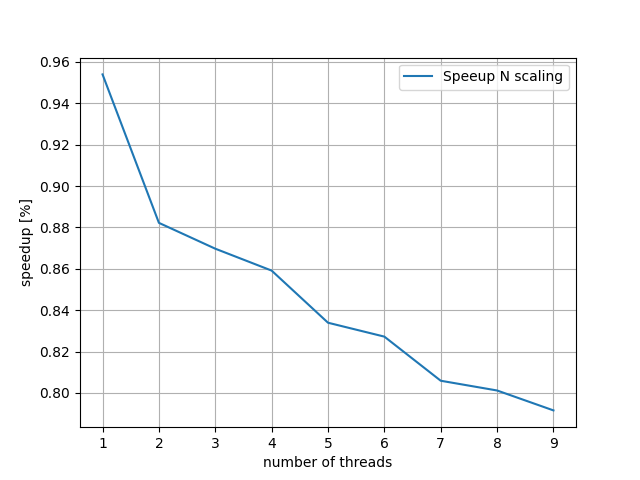
\includegraphics[width = 0.8\textwidth]{imgs/iospeedup.png}
    \captionof{figure}{speedup on the ionosphere testbench}
    \label{fig:iospeedup}
  \end{center}

  The hamerly algorithm with 1 thread still be much faster than the lloyd version but, increasing the number of threads the speedup starts to become lower.

\end{minipage}
\end{document}